
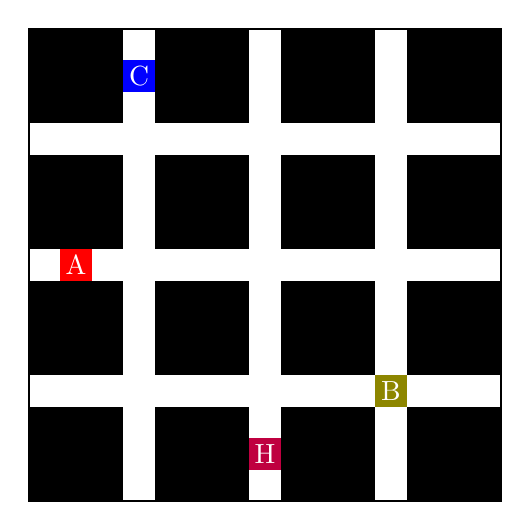
\begin{tikzpicture}[scale=0.4]
    % grid
    %\draw[step=1cm,gray] (0,0) grid (15, 15);
    % walls
    \fill[black] (0,0) rectangle ++ (3,3); 
    \fill[black] (4,0) rectangle ++ (3,3); 
    \fill[black] (8,0) rectangle ++ (3,3); 
    \fill[black] (12,0) rectangle ++ (3,3); 

    \fill[black] (0,4) rectangle ++ (3,3); 
    \fill[black] (4,4) rectangle ++ (3,3); 
    \fill[black] (8,4) rectangle ++ (3,3); 
    \fill[black] (12,4) rectangle ++ (3,3);

    \fill[black] (0, 4) rectangle ++ (3,3); 
    \fill[black] (4, 4) rectangle ++ (3,3); 
    \fill[black] (8, 4) rectangle ++ (3,3); 
    \fill[black] (12,4) rectangle ++ (3,3);

    \fill[black] (0,8) rectangle ++ (3,3); 
    \fill[black] (4,8) rectangle ++ (3,3); 
    \fill[black] (8,8) rectangle ++ (3,3); 
    \fill[black] (12,8) rectangle ++ (3,3);

    \fill[black] (0,12) rectangle ++ (3,3); 
    \fill[black] (4,12) rectangle ++ (3,3); 
    \fill[black] (8,12) rectangle ++ (3,3); 
    \fill[black] (12,12) rectangle ++ (3,3);

    \fill[red] (1,7) rectangle ++ (1,1);
    \node at (1.5,7.5) {\color{white} A};
    \fill[blue] (3,13) rectangle ++ (1,1);
    \node at (3.5,13.5) {\color{white} C};
    \fill[olive] (11,3) rectangle ++ (1,1);
    \node at (11.5,3.5) {\color{white} B};
    \fill[purple] (7,1) rectangle ++ (1,1);
    \node at (7.5,1.5) {\color{white} H};

    % Symbols

    % agent
    % \node at (3.5,1.5) {\agent};
    % \draw[ultra thick, ->, >=stealth, draw=blue!70!white] (2.5,1.9) -- (2.5,2.5) -- (1.5,2.5) -- (1.5,3.5) -- (2.5,3.5) -- (2.5,5.5) -- (1.5,5.5) -- (1.5,6.5) -- (2.5,6.5) -- (2.5,7.5) -- (3.5,7.5) -- (3.5,6.8);
    % \draw[ultra thick, ->, >=stealth, draw=blue!70!white] (3.8,6.5) -- (4.3,6.5) -- (4.3,4.8);

    % Outer box
    \draw[ thick] (0,0) rectangle (15,15);

\end{tikzpicture}